%-------------------------------------------------------------------------------
% qt_portmidi
%-------------------------------------------------------------------------------
%
% \file        qt_portmidi.tex
% \library     Documents
% \author      Chris Ahlstrom
% \date        2018-05-28
% \update      2018-10-05
% \version     $Revision$
% \license     $XPC_GPL_LICENSE$
%
%     Provides a discussion of the Qt 5 GUI and portmidi, along with a Windows
%     implementation that Seq66 supports.
%
%     However, the Qt user-interface can be combine with the more powerful
%     Rtmidi framework in the Linux version.
%
%-------------------------------------------------------------------------------

\section{Seq66 Qt 5 and Windows}
\label{sec:qt_portmidi}

   With version 0.95.1 and above,
   \textsl{Seq66} provides builds using
   the \textsl{Qt 5} GUI framework and a modified version of the
   PortMidi framework (it cleans up the code and removes the need for
   \textsl{Java}).
   With this additional work, we now have ...
   \index{Windows}
   \index{Seq66 for Windows}
   \index{qpseq66.exe}
   \textsl{Seq66 for Windows}.

   In \textsl{Linux}, the Qt 5 user-interface can be used with either the
   modified \textsl{PortMidi} library or the more powerful modified
   \textsl{RtMidi} library.

   The Qt 5 user-interface is similar
   the \textsl{Kepler34} project \cite{kepler34}.
   But it uses the internal functions of \textsl{Seq66} and adds a
   number of features not present in \textsl{Kepler34}.
   The Qt version has a tabbed interface, plus some separate windows,
   and different ways of handling the main
   window (the "Live" tab), the performance window (the "Song" tab), and the
   editing window (the "Edit" tab).
   It adds an "Events" tab and a "Playlists" tab.
   For portability reasons, the Qt user-interface will eventually be the
   \textsl{official} version for \textsl{Seq66}.
%  It will eventually be the main version of \textsl{Seq66},
%  simply because Qt 5 has fewer portability issues than Gtkmm-3.

   There is still some \textsl{Seq66} functionality that
   the Qt 5 version lacks:

   \begin{enumerate}
      \item No support for the special coloring of empty pattern slots
         or the pattern currently being edited. A low priority.
      \item A reduced-functionality options/preferences dialog, lacking an
         editor for keystroke commands.
      \item Keystroke support is not as comprehensive as the Linux version.
      \item Modified support for multi-wid.  The Qt interface allows
         for any number of external live frames.
         An arbitrary number of sets (banks) can be shown at once,
         each in its own window.  The window in focus is the active set.
   \end{enumerate}

   We are incorporating existing \textsl{Seq66} user-interface
   features into this Qt 5 version as time and bug-fixes allow.
   With version 0.96.0, we have improved the Qt/Windows version by adding the
   following features:

   \begin{enumerate}
      \item An external pattern editor has been added that matches
         the Gtkmm-2.4 \textsl{Seq66} pattern editor.  It supports
         background sequences, chord entry, event merging and extension,
         scales, snap, etc.  The tabbed pattern editor is still in place, but,
         due to space, it will never support all of the features of the
         external window.
      \item The LFO (low-frequency oscillator) window can be
         called up from the external pattern editor.
      \item The song/performance/trigger editor has been improved, and also
         made available as an external window.
      \item The pattern and song editors now have better support for zooming
         via keystrokes.
      \item A playlist tab has been added to support the new play-list
         functionality.  This tab is still a work in progress.
         See section \sectionref{sec:playlist}.
   \end{enumerate}

   Some ill-advised features from \textsl{Seq66} will not be migrated.
   Ultimately, we want to replace the Gtkmm-2.4 user-interface completely.
   But this is awhile down the road.
   There are a number of alternate versions of \textsl{Seq66} using
   PortMidi:

   \begin{enumerate}
      \item A Gtkmm-2.4 user-interface and PortMidi.  This version is
         Linux-only, and is useful for debugging the internal PortMidi code
         without worrying about the Qt 5 user-interface.
      \item A Qt 5 user-interface and PortMidi on Linux.  This version is
         useful for people who like to experiment, and for debugging Qt 5 and
         PortMidi issues at the same time.
      \item A Qt 5 user-interface and PortMidi on Windows.  This version is
         basically working, but takes some special setup.
         See \sectionref{subsec:qt_portmidi_windows_setup} for details.
   \end{enumerate}

   We also have code in place to support
   \index{Mac OSX}
   \textsl{Mac OSX},
   but currently have no OSX system on which to build and test this
   code.  \textbf{HELP WANTED!}

   In the following sections, we cover the basic differences between the
   Gtkmm-2.4 and Qt 5 versions of the application, as well as how to set up
   \textsl{Seq66 for Windows}.
   We will not show all of the user-interface elements, but we will mention
   important differences one will find.

\subsection{The Qt 5 User Interface}
\label{subsec:qt_portmidi_qt5_user_interface}

   The Qt 5 version of \textsl{Seq66} has an executable name of
   \texttt{qpseq66} (Linux) or \texttt{qpseq66.exe} (Windows).
   It is also possible to build a Qt 5 version with the RtMidi interface
   (\texttt{qseq66}), and
   that will ultimately become the default version for Linux.
   To keep explanations simple, we will refer to the Qt 5 version of
   \textsl{Seq66}, using the \textsl{PortMidi} engine,
   as \textbf{qpseq66}.
   The Gtkmm-2.4/RtMidi version (Linux only) will be referred to as
   \textbf{seq66}.

   Here is a screenshot of the main user-interface of \textsl{qpseq66}, with
   some of the patterns colored for emphasis.

\begin{figure}[H]
   \centering 
%  \includegraphics[scale=0.75]{kepler34/qt5-main-window-linux.png}
   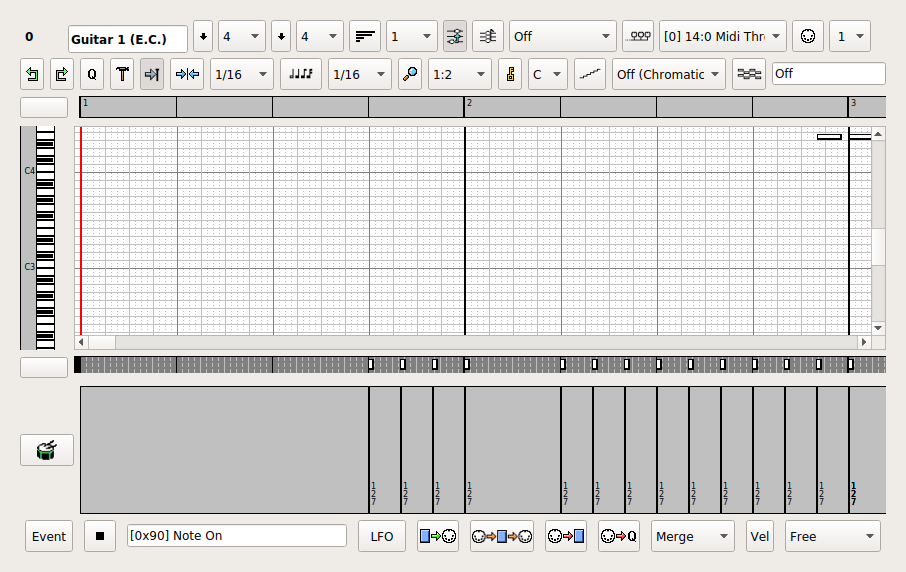
\includegraphics[scale=0.65]{roll.png}
   \caption{Qt 5 Main Window, Linux}
   \label{fig:qt5_main_window_linux}
\end{figure}

   Note the difference in layout from the Gtkmm-2.4 version.
   Also notice that some controls from the Gtkmm-2.4 version are missing.
   Some of these missing items will ultimately be added.

   There are some issues, in our opinion, with the \textsl{Kepler34} coloring
   under various situations (e.g. muting and queuing).  So we have adapted the
   \texttt{grid\_style} option in the "usr" configuration file so that, if set
   to "1", the slots look more like the Gtkmm-2.4 version of the slots:

\begin{figure}[H]
   \centering 
%  \includegraphics[scale=0.75]{kepler34/qt5-main-window-slots-gtkstyle.png}
   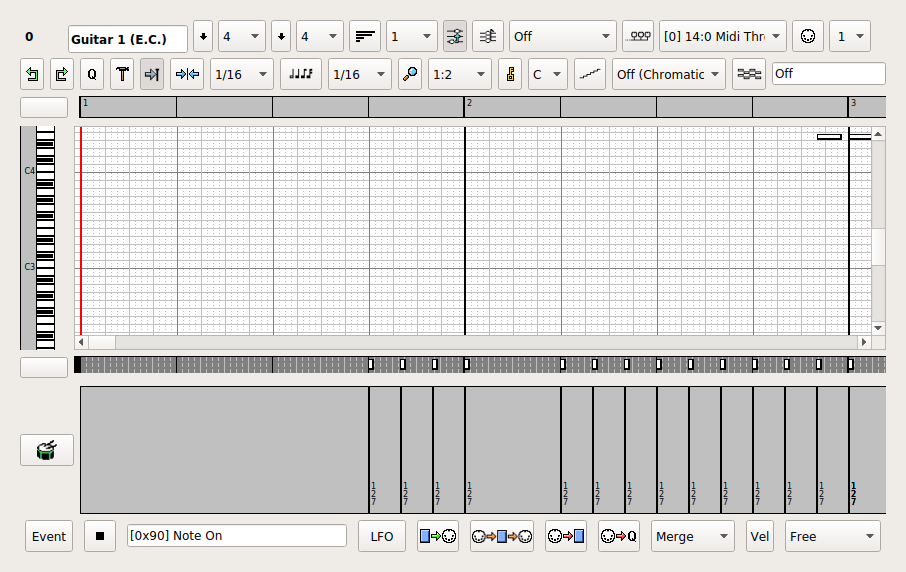
\includegraphics[scale=0.65]{roll.png}
   \caption{Qt 5 Slots in Gtk Style}
   \label{fig:qt5_main_window_slots_gtkstyle}
\end{figure}

   In this style, the outer border is either white (muted) or black (unmuted).
   Also, queuing is indicated in the legacy manner (the central box is colored
   gray), rather than with a black frame drawn around the slot.
   Choose which style you like, and send feedback about what changes would
   be desirable for either style.

%  Here is a similar screenshot in Windows 10.
%
% \begin{figure}[H]
%  \centering 
%  \includegraphics[scale=0.75]{kepler34/qt5-main-window-windows.png}
%  \caption{Qt 5 Main Window, Windows 10}
%  \label{fig:qt5_main_window_windows}
% \end{figure}

   Apart from different window decoration, the Windows version looks
   the same.  Coding an application for both Windows and Linux is very
   instructive, and can improve the overall code significantly.  It certainly
   forced us to add some new features to handle the operating-system
   differences!

\subsubsection{Qt 5 Live Slot Menu}
\label{subsubsec:qt_portmidi_qt5_live_slot_menu}

   The Qt 5 version of the right-click pattern/slot menu is slightly different
   from the Gtkmm-2.4 version.

\begin{figure}[H]
   \centering 
%  \includegraphics[scale=0.75]{kepler34/qt5-live-frame-slot-menu.png}
   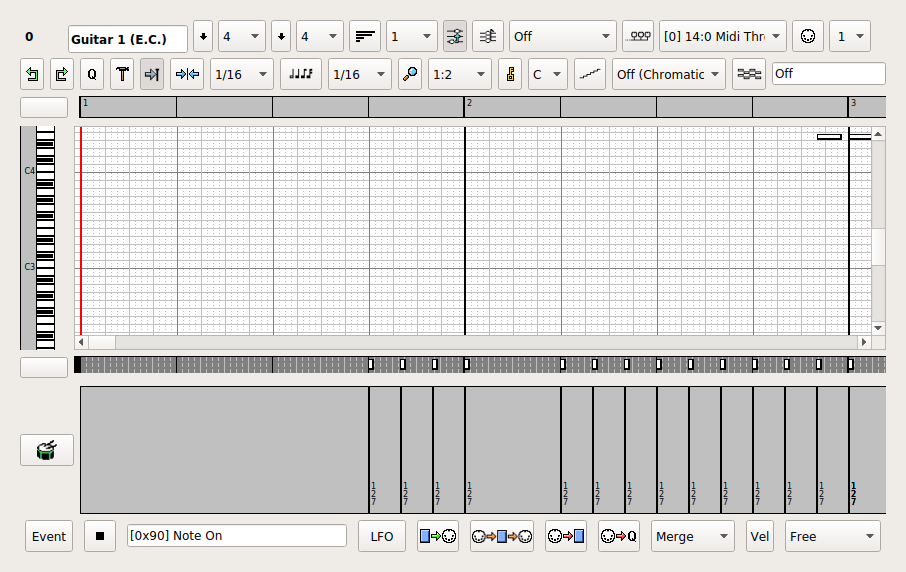
\includegraphics[scale=0.65]{roll.png}
   \caption{Qt 5 Slot Menu}
   \label{fig:qt5_main_window_slot_menu}
\end{figure}

   It lets one add an external window for the pattern slots (live-frame),
   and lets one open a pattern editor in a tab or in an external window.
   It lets one edit events textually in a tab.  Here are the menu entries to
   describe:
   
   \begin{enumber}
      \item \textbf{New pattern}
      \item \textbf{External live frame}
      \item \textbf{Edit pattern in tab}
      \item \textbf{Edit pattern in window}
      \item \textbf{Edit events in tab}
      \item \textbf{Copy pattern}
      \item \textbf{Cut pattern}
      \item \textbf{Delete pattern}
   \end{enumber}

   Let's describe them.

   \setcounter{ItemCounter}{0}      % Reset the ItemCounter for this list.

   \itempar{New pattern}{qt!new pattern}
      Creates a new pattern in the slot.
      If there is already a pattern there, the user is prompted about a
      sequence already present, with a yes/no question about overwriting it and
      creating a new blank sequence.

   \itempar{External live frame}{qt!external live frame}
      With Qt 5, we decided not to reimplement the Gtkmm-2.4 version's
      "multiwid" features, which allows one to specify a matrix of screen-sets.
      This option creates an additional "Live" frame, which is external to the
      Live frame tab.  This live-frame shows the set/bank corresponding to the
      slot number (tricky!) over which the menu was opened.  This won't work if
      used on a higher set.  When an external live-frame has focus, it
      represents the \textsl{active set/bank}.  The active set is shown in the
      main window in the \textbf{Active Set} field, just to be clear.

\begin{figure}[H]
   \centering 
%  \includegraphics[scale=0.75]{kepler34/qt5-external-live-frame.png}
   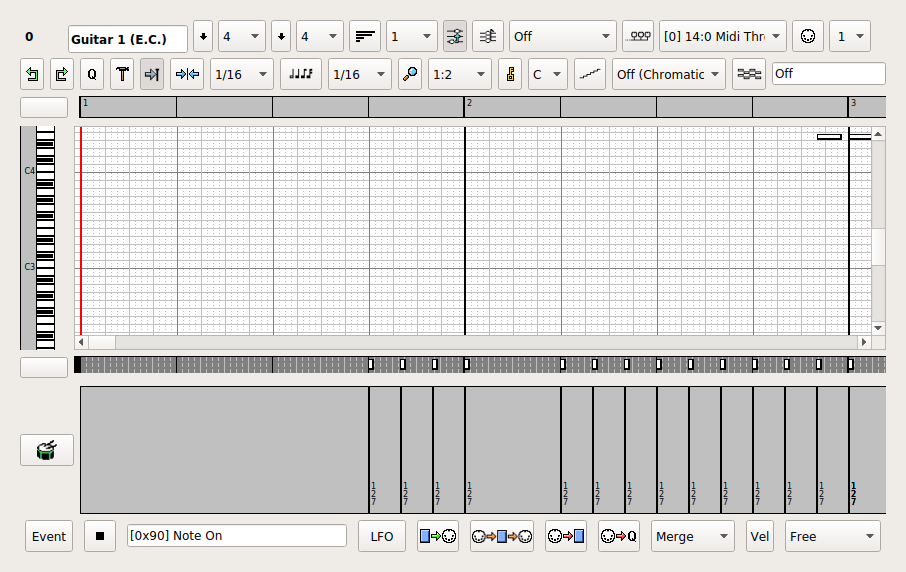
\includegraphics[scale=0.65]{roll.png}
   \caption{Qt 5 External Live Frame}
   \label{fig:qt5_main_window_external_live_frame}
\end{figure}

   \itempar{Edit pattern in tab}{qt!edit pattern in tab}
      Sets up a pattern editor in the "Edit" tab.  This editor is not as
      versatile as the external-window pattern editor described in the next
      section.

   \itempar{Edit pattern in window}{qt!edit pattern in window}
      Sets up a pattern editor a separate window.  This pattern editor works a
      lot like the Gtkmm-2.4 version, though it does not support the "fruity"
      mode of editing.

   \itempar{Edit events in tab}{qt!edit events in tab}
      Sets up an event editor in the "Edit" tab.  This editor is a basic editor
      and mostly useful for finding and deleting unwanted events, or adding
      events that are not otherwise available.

   \itempar{Copy pattern}{qt!copy pattern}
      Copies the selected pattern.

   \itempar{Cut pattern}{qt!cut pattern}
      Cuts (and copies) the selected pattern.

   \itempar{Delete pattern}{qt!delete pattern}
      Deletes the selected pattern.

\subsubsection{Qt 5 Live Tab}
\label{subsubsec:qt_portmidi_qt5_live_tab}

   The \textbf{Live} tab of \textsl{qpseq66}, as shown above, is very similar
   to the \textsl{seq66} version.  It supports the
   varisets mode (the alternate row-by-column sizes of \textsl{seq66}).
   In addition, external versions of the Live frame can be instantiated outside
   of the main window, so that the user can
   view and work with a number of set/banks at the same time.

   The size of this window can be changed to a certain degree via
   the command-line option \texttt{--option scale=x.y}, where \texttt{x.y} can
   range from 0.4 to 3.0.  This can be made permanent via the
   \texttt{window-scale} setting in the "usr" file.
   For example, these two options should be used together:
   \texttt{-o sets=8x8 -o scale=1.5}.  Experiment with varying values for these
   options.

   In fact, all of the tabs except for the \textbf{Events} and
   \textbf{Playlist}
   tabs will expand properly to
   use additional space if the application is resized, whether by a
   command-line option or by dragging a corner of the window.

\subsubsection{Qt 5 Song Tab}
\label{subsubsec:qt_portmidi_qt5_song_tab}

\begin{figure}[H]
   \centering 
%  \includegraphics[scale=0.75]{kepler34/qt5-song-window-linux.png}
   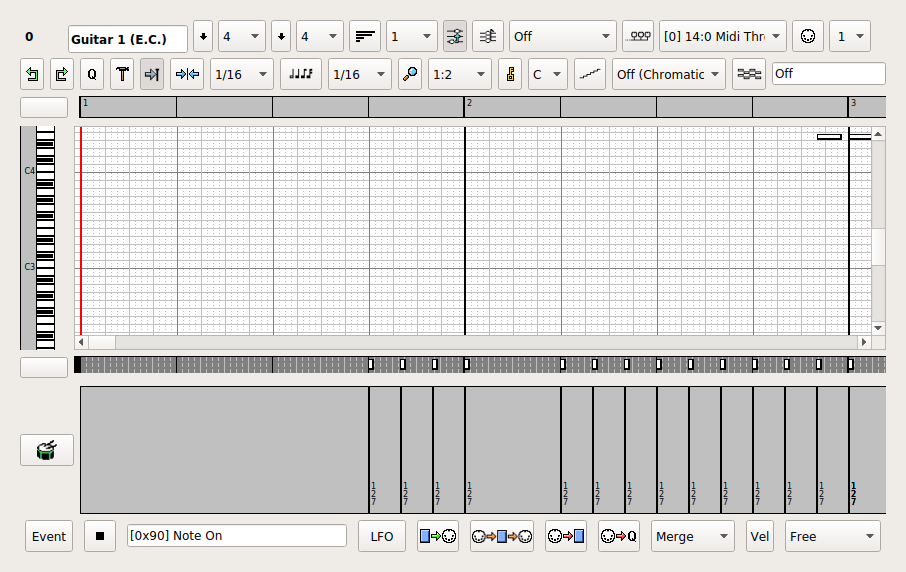
\includegraphics[scale=0.65]{roll.png}
   \caption{Qt 5 Song Window, Linux}
   \label{fig:qt5_song_window_linux}
\end{figure}

   This window is very similar to the \textsl{seq66} version.
   Additional features may be added as time goes on.  In addition,
   this frame can be opened in its own external window by
   pressing the "Song Editor" button at the bottom of the main window.

\subsubsection{Qt 5 Edit Tab}
\label{subsubsec:qt_portmidi_qt5_edit_tab}

\begin{figure}[H]
   \centering 
%  \includegraphics[scale=0.75]{kepler34/qt5-edit-window-linux.png}
%  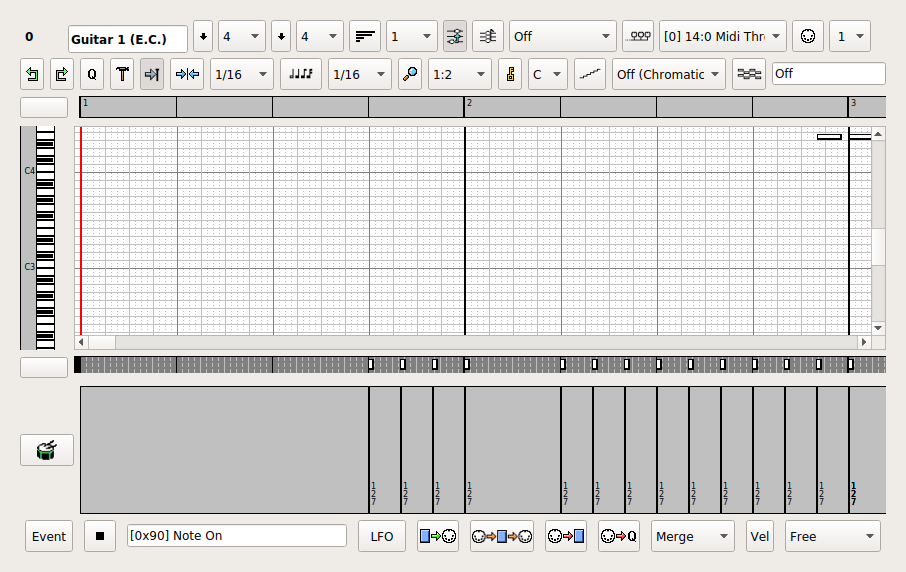
\includegraphics[scale=0.65]{roll.png}
   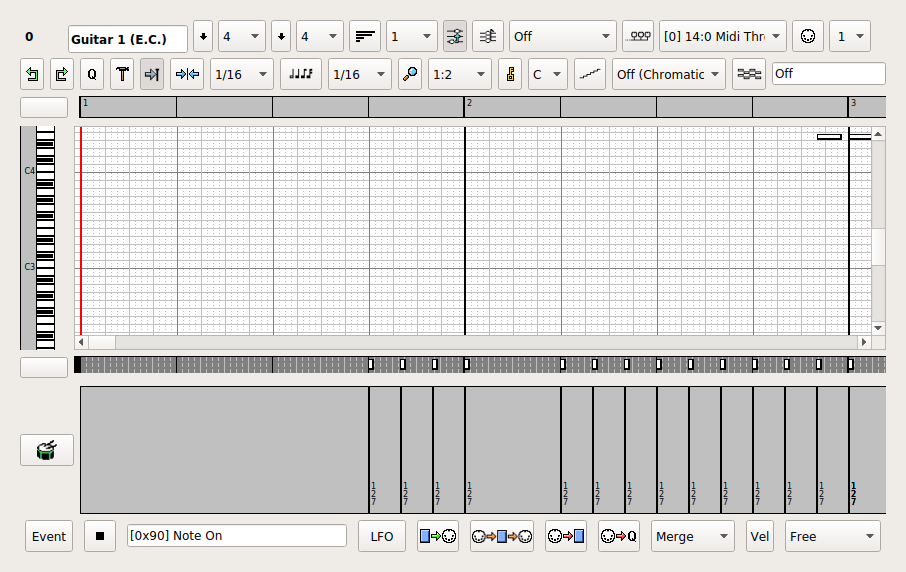
\includegraphics[scale=0.65]{roll.png}
   \caption{Qt 5 Edit Window, Linux}
   \label{fig:qt5_edit_window_linux}
\end{figure}

   This version of the pattern editor is a bit behind
   \textsl{seq66} for features.  There really isn't enough space in the
   main window for all the features of the \textsl{Seq66} pattern editor.
   Note that the event-data editor panel is not visible here.
   One must scroll down to the bottom of the window to see it and use it.
   Note that that the \textbf{LFO} window is not accessible here.
   Finally, note that the note heights and vertical grid spacing are
   modifiable via a key-height option, which is a feature the Gtkmm-2.4
   user-interface does not offer.

   With version 0.95.1, the pattern/slot popup menu has an option to open the
   pattern in an external window that has a lot more features than the
   pattern editor in the tab.  It also has a different scrolling mechanism,
   more like that of \textsl{seq66}.
   Note that only one of the tab/external pattern
   editors can be shown at the same time for a given pattern.
   This pattern editor is pretty much identical to the Gtkmm-2.4 version,
   except that it does not provide a "fruity" mode of mouse usage.
   Sorry.

\subsubsection{Qt 5 Events Tab}
\label{subsubsec:qt_portmidi_qt5_events_tab}

\begin{figure}[H]
   \centering 
%  \includegraphics[scale=0.75]{kepler34/qt5-event-editor.png}
   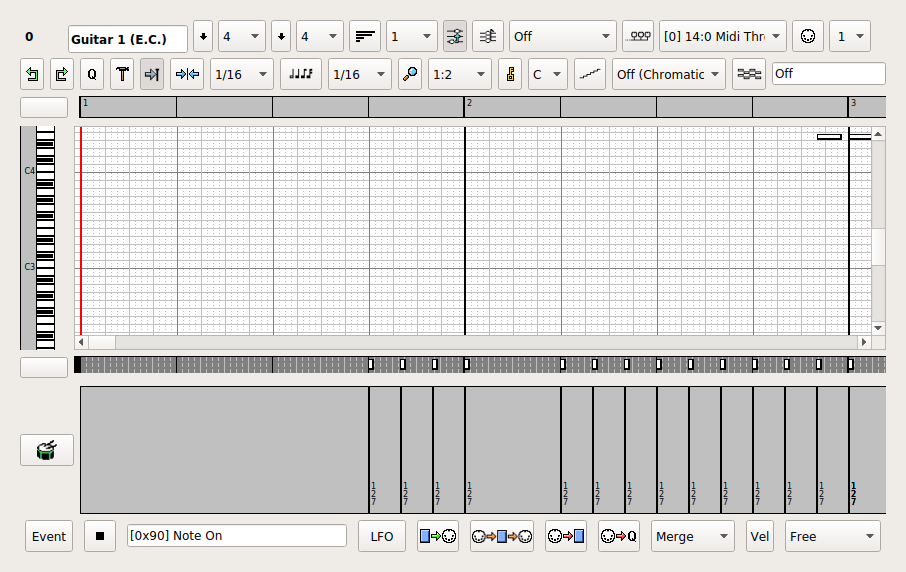
\includegraphics[scale=0.65]{roll.png}
   \caption{Qt 5 Events Window}
   \label{fig:qt5_events_window}
\end{figure}

   This window works a lot like \sectionref{sec:event_editor}; please see
   that section for user instructions.  Please remember that, at the present
   time, this view is meant only for viewing events and making minor tweaks to
   a pattern, such as eliminating problematic events.  It is not intended to be
   a full-featured event editor.  In particular, note that editing within each
   cell in the event table is not supported.  Event editing must be done in the
   right panel.  An event must be explicitly selected by clicking on it, before
   it can be modified or deleted.

   Also, if one adds or modifies an event to show up an the end of the pattern,
   by modifying the time stamp, the event will appear there, but the
   user-interface will remain at the current event.

\subsubsection{Qt 5 Playlist Tab}
\label{subsubsec:qt_portmidi_qt5_playlist_tab}

\begin{figure}[H]
   \centering 
%  \includegraphics[scale=0.75]{kepler34/qt5-playlist-editor.png}
   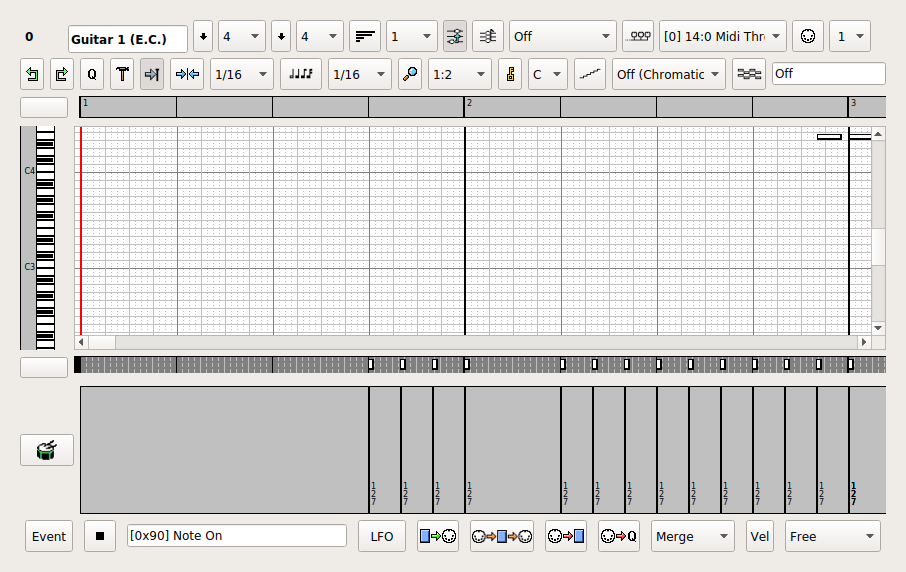
\includegraphics[scale=0.65]{roll.png}
   \caption{Qt 5 Playlist Window}
   \label{fig:qt5_playlist_window}
\end{figure}

   The play-list functionality can be viewed in this tab.
   Currently, this tab only shows the playlist items.  One can
   select a playlist, and view the song-titles in it, but
   editing and loading the play-lists and songs does not yet
   work.  One must edit the play-list file manually for now,
   and load it from the \textbf{File / Open Playlist} menu.

   Also note that the play-list title can be seen in the main live frame, 
   and that play-lists and songs-can be selected with the arrow keys in that
   window.

   See section \sectionref{sec:playlist}; there are many things that can be
   done with the playlist feature, including controlling it via MIDI events.

\subsubsection{Qt 5 Edit / Preferences}
\label{subsubsec:qt_portmidi_qt5_edit_prefs}

\begin{figure}[H]
   \centering 
%  \includegraphics[scale=0.75]{kepler34/qt5-prefs-clock-windows.png}
   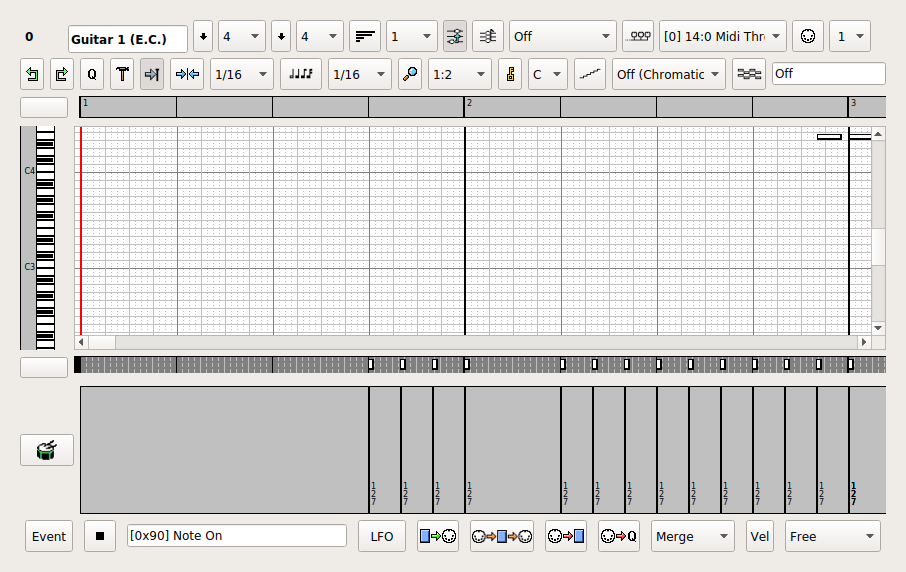
\includegraphics[scale=0.65]{roll.png}
   \caption{Qt 5 Clock Preferences, Windows}
   \label{fig:qt5_prefs_clock_windows}
\end{figure}

   In a newer version of this document, we will show the other preferences
   tabs.  There are many tabs we still need to add to this dialog.
   In particular, be sure to go to the \textbf{MIDI Input} tab and
   make sure that your desired input device (e.g. a MIDI keyboard) are shown
   and are enabled.
   Since the Qt GUI pretty much hardwires the keystrokes used for various
   functions such as muting and queuing, we might not provided a keystroke
   mapping editor.  To be determined.
   In any event, many of the keystrokes configured in the "rc" file are
   supported, but one might have to edit the "rc" file directly, keeping
   in mind that it uses Gtkmm-2.4 conventions for keystrokes.
   \textsl{Linux} users can edit the keystrokes and copy the "rc" configuration
   into the Qt 5 "rc" file, \texttt{qpseq66.rc}.

\subsection{Seq66 Windows Setup}
\label{subsec:qt_portmidi_windows_setup}

   \textsl{Seq66 for Windows} (\textsl{qpseq66}) can be installed
   as a portable Zip package anywhere the user desires.  The package is
   self-contained, and contains all the the DLLs needed to run the program.
   \textsl{qpseq66} can also be installed via an NSIS-based installer,
   such as \texttt{seq66\_setup\_0.96.0-0.exe}.

\subsubsection{Seq66 Windows Issues}
\label{subsubsec:qt_portmidi_windows_setup_issues}

    When first starting \textsl{qpseq66} on \textsl{Windows}, one might
    experience some issues.  One issue is that the \textsl{Microsoft MIDI
    Mapper}, rumored to be removed in \textsl{Windows 8} and beyond, is still
    detected by the internal PortMidi library used in \textsl{qpseq66}.
    Another issue is that the built-in \textsl{Microsoft} wave-table
    synthesizer might not be accessible.

    We installed the
    \textsl{CoolSoft MIDIMapper} (\cite{midimapper}) and
    \textsl{VirtualMIDISYnth} (\cite{midisynth}) to try to get
    around these issues, and tried to turn off the
    \texttt{Windows System Sound} setup of
    \textsl{"Allow applications to restrict access to this device."}
    But we still had
    inaccessible devices, and the resulting errors would cause
    \textsl{qpseq66} to
    abort.  So we had to spend a lot of time adding support for
    the disabling of
    inaccessible ports, and saving and restoring the "rc" setup properly
    in the face of device-access errors.

    Here is some output logging on our Windows, generated using the
    \texttt{qpseq66} command-line option
    \texttt{-o log=virtualmidi.log}, which dumps the log file into

   \begin{verbatim}
       C:/Users/chris/AppData/Local/seq66/virtualmidi.log
   \end{verbatim}

\begin{verbatim}
   qpseq66 
   C:/Users/chris/AppData/Local/seq66/virtualmidi.log 
   2018-05-13 09:06:58 
   [MIDIMAPPER] 'mapper in : midiInGetDevCaps() error for device 'MIDIMAPPER':
      'The specified device identifier is out of range'
   pm_winmm_general_inputs(): no input devices
   PortMidi MMSystem 0: Microsoft MIDI Mapper output opened
   PortMidi MMSystem 1: CoolSoft MIDIMapper output closed
   PortMidi MMSystem 2: Microsoft GS Wavetable Synth output opened
   PortMidi MMSystem 3: VirtualMIDISynth #1 output closed
   [Opened MIDI file,
      'C:/Users/chris/Documents/Home/seq66/data/b4uacuse-gm-patchless.midi']
   [Writing rc configuration C:/Users/chris/AppData/Local/seq66/qpseq66.rc]
   PortMidi call failed: [-1] 'Bad pointer'
   PortMidi call failed: [-1] 'Bad pointer'
   Begin closing open devices...
   Warning: devices were left open. They have been closed.
\end{verbatim}

    By disabling the "closed" devices in the \texttt{qpseq66.rc} file,
    we are able to start.  Here are the settings:

\begin{verbatim}
      5    # number of MIDI clocks/busses
      # Output buss name: [0] 0:0 PortMidi:Microsoft MIDI Mapper
      0 0    # buss number, clock status
      # Output buss name: [1] 1:2 PortMidi:CoolSoft MIDIMapper
      1 -1    # buss number, clock status
      # Output buss name: [2] 2:3 PortMidi:Microsoft GS Wavetable Synth
      2 0    # buss number, clock status
      # Output buss name: [3] 3:4 PortMidi:VirtualMIDISynth #1
      3 -1    # buss number, clock status
\end{verbatim}

   These settings tell \textsl{Seq66} to ignore output busses 1 and 3,
   in order to allow it to start without error.

    We still have some minor issues at start up and at exit, but are now able
    to play a tune on the wavetable synthesizer using the
    \texttt{--bus 2} option, which forces output to PortMidi buss 2,
    "Microsoft GS Wavetable Synth".

    If an error occurs at start-up, a file called \texttt{erroneous.rc} is
    written to the configuration directory, and can be examined for issues with
    ports.

\subsubsection{Seq66 Windows Configuration Files}
\label{subsubsec:qt_portmidi_windows_setup_config}

    When you first run \textsl{qpseq66}
    on \textsl{Windows}, it will create a new configuration
    file, with inaccessible devices denoted in the
    \texttt{[midi-clock]} section of
    \texttt{C:/Users/username/AppData/Local/seq66/qpseq66.rc}
    by a \texttt{-1} value.

    On \textsl{Linux},
    the normal directory location of the \textsl{Seq66} configuration
    files is

\begin{verbatim}
    /home/username/.config/seq66
\end{verbatim}

   There are various configuration file names, depending on the name of the
   built application:

\begin{verbatim}
        seq66.rc      The RtMidi Native ALSA/JACK version.
        seq66.usr     The same, but for user-interface settings.
        seq66portmidi.rc    The PortMidi Gtkmm 2.4 version.
        seq66portmidi.usr   The same, but for user-interface settings.
        qseq66.rc           The RtMidi Qt 5 version for Linux.
        qseq66.usr          The same, but for user-interface settings.
        qpseq66.rc          The PortMidi Qt 5 version for Windows.
        qpseq66.usr         The same, but for user-interface settings.
\end{verbatim}

    On \textsl{Windows}, the conventional configuration file
    location is different:
    
\begin{verbatim}
    C:/Users/username/AppData/Local/seq66
\end{verbatim}

    The files are:

\begin{verbatim}
        qpseq66.rc          The PortMidi Qt 5 version for Windows.
        qpseq66.usr         The same, but for some user-interface settings.
\end{verbatim}

    Typical of \textsl{Microsoft}, access to the \texttt{AppData} directory
    is not obvious... "we cannot have users monkeying with the configuration".
    To access \texttt{AppData}, highlight the user-name directory
    (e.g. \texttt{C:/Users/chris}, then append
    "AppData" to the end of it.  Voila! It is now visible in
    \textsl{Windows Explorer}.
    It is a Windows \textsl{thang}.
    Then click on the \texttt{seq66} directory.
    Open \texttt{qpseq66.rc} and see what is in it (scroll down a bit):

\begin{verbatim}
    [midi-clock]
    2    # number of MIDI clocks/busses
    # Output buss name: [0] 0:0 PortMidi:Microsoft MIDI Mapper
    0 0  # buss number, clock status
    # Output buss name: [2] 1:1 PortMidi:Microsoft GS Wavetable Synth (virtual)
    1 0  # buss number, clock status
    # Output buss name: [3] 1:1 PortMidi:nanoKEY2
    2 0  # buss number, clock status
\end{verbatim}
    
\begin{verbatim}
    [midi-input]
    1    # number of input MIDI busses
    # The first number is the port number, and the second number
    # indicates whether it is disabled (0), or enabled (1).
    # [1] 0:1 PortMidi:nanoKEY2
    0 1
\end{verbatim}

   These settings can be accessed via
   \textbf{Edit / Preferences / MIDI Clock} and
   \textbf{Edit / Preferences / MIDI Input} to
	alter the ports accessible, in the \textsl{Windows}
   version of \textsl{Seq66}.
   The operating system may have some devices locked out, though.
   Generally, the device needs to have a "System Sound" setting that allows an
   application to grab exclusive access to the device.
   For now, do a web search for this error message, if you have issues:

\begin{verbatim}
   'The specified device is already in use.  Wait until it is free, and then
   try again.'
\end{verbatim}

%-------------------------------------------------------------------------------
% vim: ts=3 sw=3 et ft=tex
%-------------------------------------------------------------------------------
